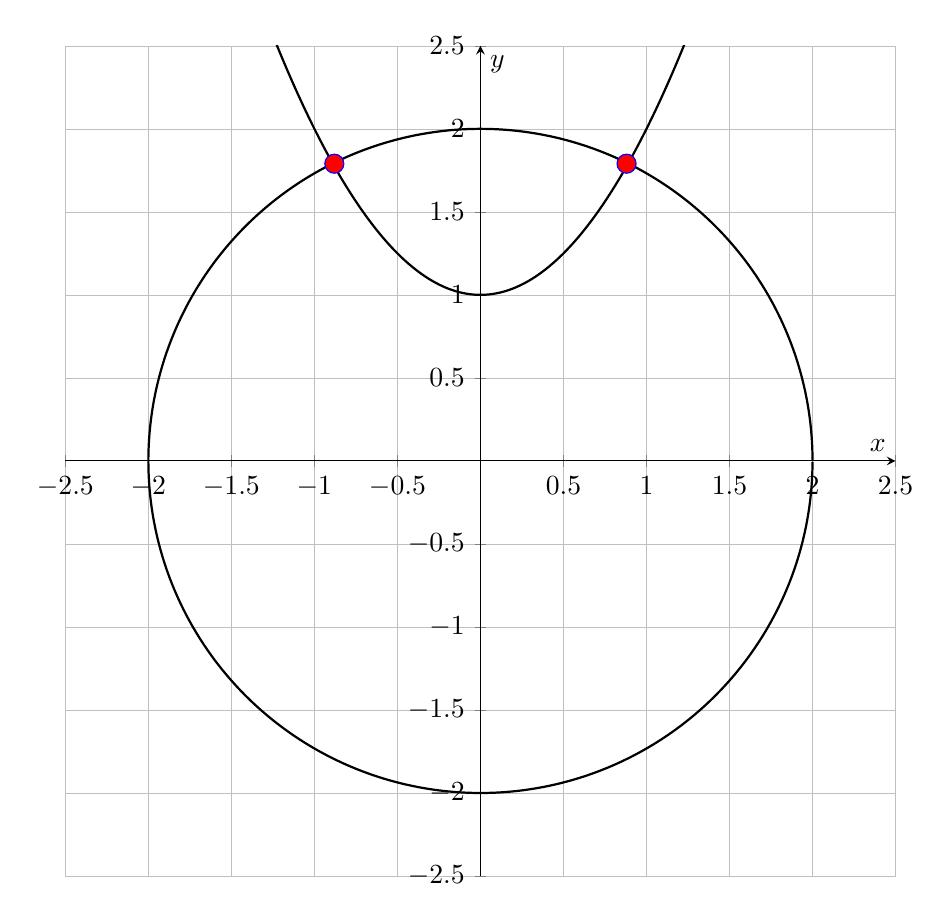
\begin{tikzpicture}
    \begin{axis}[
      axis lines=middle,
      xmin=-2.5,xmax=2.5,
      ymin=-2.5,ymax=2.5,
      xlabel={\(x\)},
      ylabel={\(y\)},
      grid=both,
      grid style={line width=.1pt, draw=gray!20},
      major grid style={line width=.2pt,draw=gray!50},
      width=\textwidth, height=\textwidth
    ]
    
    \coordinate (r0) at (0.88,1.79);
    \coordinate (r1) at (-0.88,1.79);
    
    
    % Draw the circle x^2 + y^2 = 4
    \addplot [samples=200, domain=0:2*3.14, smooth, thick] ({2*cos(deg(x))}, {2*sin(deg(x))});
    
    % Draw the parabola y = x^2 + 1
    \addplot [samples=200, domain=-2:2, smooth, thick] {x^2 + 1};
    
    \draw[fill=red, draw=blue] (r0) circle (0.01\textwidth);
    \draw[fill=red, draw=blue] (r1) circle (0.01\textwidth);
    
    \end{axis}
    \end{tikzpicture}